\chapter{Optimization Algorithm}
\label{chapter:optimization}

An optimization problem is any problem where a function $f:X \rightarrow Y$ is given, and we search for the point $x \in X$ such that $f(x)$ is minimal or maximal. Obviously the minimum or maximum must not exist, as the example $f: (0, 1) \rightarrow \mathbb{R}, x \mapsto x$ demonstrates by not having either. Investigating conditions on $X$, $Y$ and $f$ such that a minimum or maximum exists is mathematically interesting. However, when implementing an optimization algorithm the true minimum or maximum can sometimes not be found even if it exists and is instead replaced by a sufficiently good approximation.

\section{Gradient Descent}

An iterative algorithm for finding the minimum of a differentiable function $f: \mathbb{R}^n \rightarrow \mathbb{R}$ is gradient descent. As the name suggests it uses information of the gradient $\nabla f$. Locally the negative gradient always points into the direction of greatest descent. The idea is to follow this direction for the next guess of the minimum. The pseudocode of this approach is given below.

\begin{algorithm}[H] \label{alg:gradient_descent}
	\SetAlgoLined
	\DontPrintSemicolon
	\LinesNumbered
	\SetKwInOut{Input}{input}
	\SetKwInOut{Output}{output}
	\caption{Gradient Descent}
	
	\Input{$f: \mathbb{R}^n \rightarrow \mathbb{R}$ ... differentiable, $x_0 \in \mathbb{R}^n$}
	\Output{$x \in \mathbb{R}^n$}
	\BlankLine
	\Begin{
		\For{$n=0$ \KwTo max\_iterations}{
			\If{improvement is smaller than threshold}{
				break\;
			}
			set or calculate step size $\gamma_n$\;
			$x_{n+1} = x_n - \gamma_n \nabla f(x_n)$\;
		}
		$x = x_n$\;
	}
\end{algorithm}
\vspace{1cm}

If we consider a function with a local minimum, that is not a global minimum, gradient descent might not converge to the optimum. An example of such a function can be seen in figure~\ref{fig:grad_descent_global_min_not_found} along with the first few values $x_n$ of gradient descent. The starting value was chosen to not have convergence to the global minimum. For a different starting value the global minimum can be reached.

\begin{figure}[h]
	\centering
	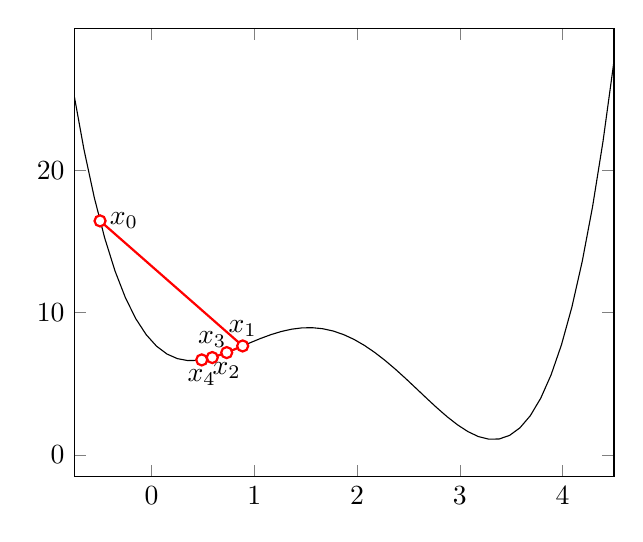
\begin{tikzpicture}
		\begin{axis}[xmin=-0.75, xmax=4.5, samples=100]
			\addplot[black] (x,x*x*x*x - 7*x*x*x + 14*x*x - 8*x + 8);
			\addplot[color=red,solid,thick,mark=*, mark options={fill=white}] 
			coordinates {
				(-0.5, 16.4375)
				(0.8875, 7.65428)
				(0.73223, 7.18773)
				(0.591558, 6.84009)
				(0.4894125, 6.67483)
			}; 
			\node [right] at (axis cs:  -0.5,  16.4375) {$x_0$};
			\node [above] at (axis cs:  0.8875, 7.65428) {$x_1$};
			\node [below] at (axis cs:  0.73223, 7.18773) {$x_2$};
			\node [above] at (axis cs:  0.591558, 6.84009) {$x_3$};
			\node [below] at (axis cs:  0.4894125, 6.67483) {$x_4$};
		\end{axis}
	\end{tikzpicture}
	\caption{The function has two local minimums. For this starting value and step size gradient descent approaches the local, but not global minimum.}
	\label{fig:grad_descent_global_min_not_found}
\end{figure}

Improvements can be made by choosing good step sizes, starting value or by starting with different values and comparing the results.

\section{Least Square Problem Algorithms}

% https://docs.scipy.org/doc/scipy/reference/generated/scipy.optimize.least_squares.html

We now focus on the Least Square Problem and give an introduction into various algorithms solving this problem.

In the example dealt with in this work we are given some data points $((x_k, y_k))_{k \in \{1, 2, ..., n\}}$ and want to find a close approximation in the form of a function $g(x, a_1, a_2, ..., a_m)$ where for every list of function parameters $a = (a_1, ..., a_m)$ we have the function $g_a(x) : \mathbb{R} \rightarrow \mathbb{R}, x \mapsto g(x, a_1, ..., a_m)$. Searching for a good approximation can be reformulated as searching for the minimum of $r(a) := \sum_{k=1}^{n} |g_a(x_k) - y_k|^2$ or any other error function. This form of optimization problem is called the Least Square Problem.

First we want to discuss some variations of the problem. Easiest to solve are linear problems. These can be formulated as the minimization of $||Ax - b||^2$, and solved using calculus by $x=(A^TA)^{-1}A^Tb$ provided the rank of $A$ is full.

Often we want to constrain the search for a minimum under some properties. For linear problems we can find a formulation as

\begin{align*}
	\text{minimize } ||Ax-b||^2 \text{ subject to } Cx=d.
\end{align*}

Finding a solution can be done by minimizing $||Ax-b||^2 + \lambda ||Cx-d||^2$ for very large $\lambda$.

General least square problems are formally given as a residual function $r_f(x)$ which tells us whether a function $f$ is a good approximation at the point $x$. We therefore want to find a way to minimize $||r_f(x)||^2$.

As $||r_f(x)||^2 \geq 0$ we can turn to the simpler problem of finding a root. However, a root must not exist, in which case we want to find the value closest to zero. This is then the minimum of the function.

Some algorithm for minimization are now discussed below.

\subsection{Gauss–Newton Algorithm}

The idea behind this algorithm is that it is easy to find the intersection with zero of a linear function. If we linearize $r:\mathbb{R}^n \rightarrow \mathbb{R}^m$ locally, we can approximate the root by finding it of the linear approximating function. This is demonstrated in figure~\ref{fig:approx_root_with_lin}.

\begin{figure}[h]
	\centering
	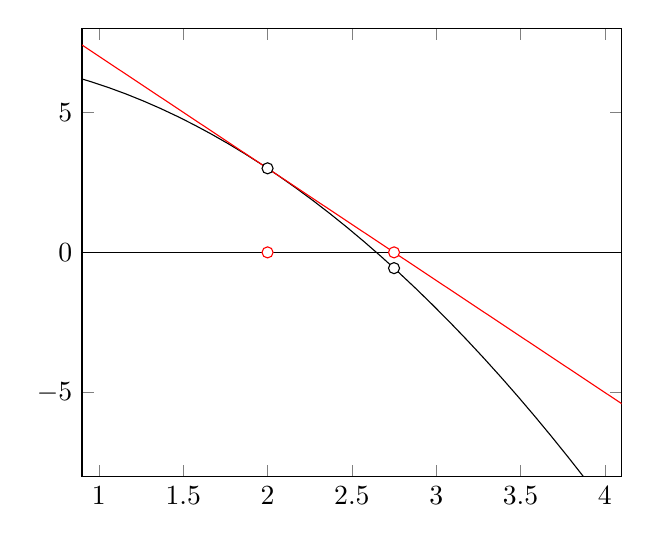
\begin{tikzpicture}
		\begin{axis}[xmin=0.9, xmax=4.1, ymin=-8, ymax=8, samples=100]
			\addplot[black] (x,-x*x + 7);
			\addplot[red] (x,-4*x+11);
			\addplot[black] (x,0);
			\addplot[color=black,only marks,mark=*, mark options={fill=white}] 
			coordinates {
				(2, 3)
				(2.75, -0.5625)
			};
			\addplot[color=red,only marks,mark=*, mark options={fill=white}] 
			coordinates {
				(2, 0)
				(2.75, 0)
			};
		\end{axis}
	\end{tikzpicture}
	\caption{By approximating the black function by a line an approximation of the root has been found.}
	\label{fig:approx_root_with_lin}
\end{figure}

Iterating this step of linear approximating gives us the Gauss-Newton Method. In figure~\ref{fig:gauss_newton_example} we can see that indeed $x_n$ seems to converge towards the root of the function.

\begin{figure}[h]
	\centering
	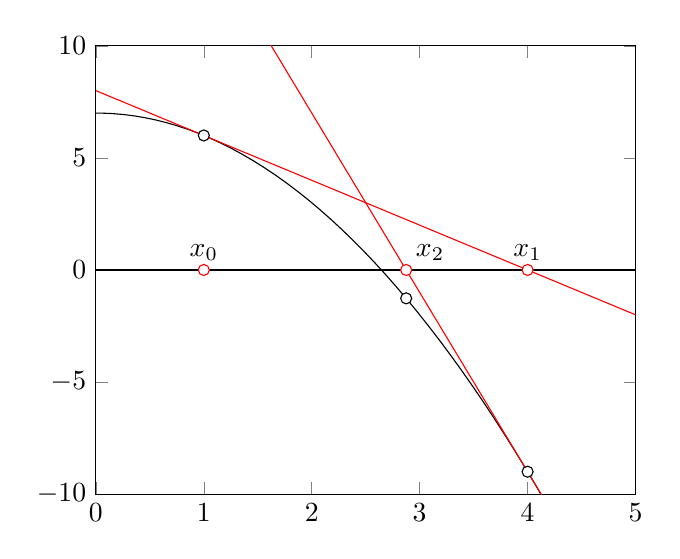
\begin{tikzpicture}
		\begin{axis}[xmin=0, xmax=5, ymin=-10, ymax=10, samples=100]
			\addplot[black] (x,-x*x + 7);
			\addplot[red] (x,-2*x+8);
			\addplot[red] (x,-8*x+23);
			\addplot[black] (x,0);
			\addplot[color=black,only marks,mark=*, mark options={fill=white}] 
			coordinates {
				(1, 6)
				(4, -9)
				(2.875, -1.265625)
			};
			\addplot[color=red,only marks,mark=*, mark options={fill=white}] 
			coordinates {
				(1, 0)
				(4, 0)
				(2.875, 0)
			};
			\node [above] at (axis cs:  1,   0) {$x_0$};
			\node [above] at (axis cs:  4,   0) {$x_1$};
			\node [above right] at (axis cs:  2.875,0) {$x_2$};
		\end{axis}
	\end{tikzpicture}
	\caption{Iteratively applying linear approximation gives the Gauss-Newton Method for approximating the root.}
	\label{fig:gauss_newton_example}
\end{figure}

Define $Dr$ as the Jacobian matrix $\left(\frac{\partial r_i}{\partial x_j}\right)_{ij}$. Using Taylor's theorem we get the linear approximation

\begin{align*}
	r(x) = r(a) + Dr(a)(x-a) + h(x)(x-a) \approx r(a) + Dr(a)(x-a) \text{ with } \lim\limits_{x\rightarrow a}h(x) = 0.
\end{align*}

Rewriting this as $r(x) \approx Ax - b$ where $A := Dr(a)$ and $b := Dr(a)a-r(a)$ gives us the algorithm for this method. As $Dr \in \mathbb{R}^{n\times m}$ we solve $Dr^T Dr x = Dr^T b$ in order to get a system with square matrix. If $n=m$ we can skip this step and get the so-called Newton algorithm as a variant.

\begin{algorithm}[H] \label{alg:gauss_newton}
	\SetAlgoLined
	\DontPrintSemicolon
	\LinesNumbered
	\SetKwInOut{Input}{input}
	\SetKwInOut{Output}{output}
	\caption{Gauss-Newton}
	
	\Input{$r: \mathbb{R}^n \rightarrow \mathbb{R}^m$ ... differentiable, $x_0 \in \mathbb{R}^n$}
	\Output{$x \in \mathbb{R}^n$}
	\BlankLine
	\Begin{
		\For{$n=0$ \KwTo max\_iterations}{
			\If{$||r(x_n)||^2$ close enough to zero or $||x_n - x_{n-1}||$ is too small}{
				break\;
			}
			Calculate $A_n := Dr(x_n)$\;
			Calculate $b_n := A_n x_n - r(x_n)$\;
			Solve $A_n^T A_n x_{n+1} = A_n^T b_n$\;
		}
		$x := x_n$\;
	}
\end{algorithm}
\vspace{1cm}

Gauss-Newton is guaranteed to find a local minimum $x$ if $r$ is twice continuously differentiable in an open convex set including $x$, $Dr$ has a full rank and the initial value is close enough to $x$.

For the example demonstrated in figure~\ref{fig:gauss_newton_fails_sin} we can see that choosing a particular starting value leads to a loop in which only two points are explored as possible roots. More extreme examples exists in which Gauss-Newton gets increasingly further away from the root, due to an increasingly flat incline the further we get from the root. One example of such a function can be seen in figure~\ref{fig:gauss_newton_fails_cubic_root}.

\begin{figure}
	\centering
	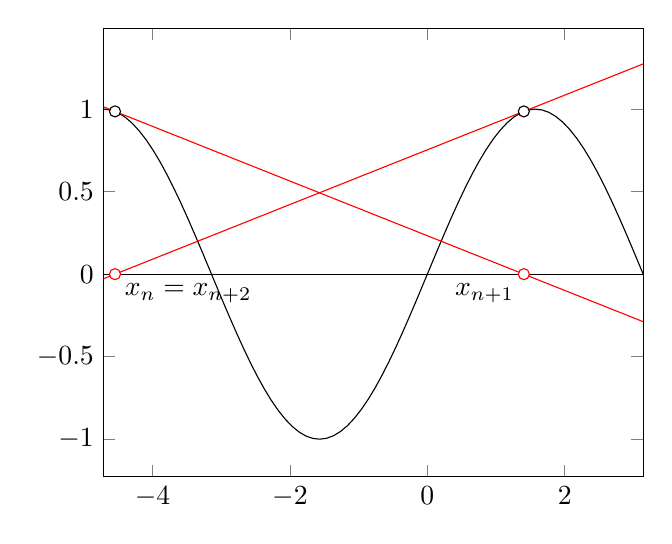
\begin{tikzpicture}
		\begin{axis}[xmin=-4.71238898, xmax=3.141592653, samples=100]
			\addplot[black] {sin(deg(x))}; 
			\addplot[red] (x,-0.165738017518283266*x+0.23274423977441288);
			\addplot[red] (x,0.16573801751814743279*x+0.75342557803057879409);
			\addplot[black] (x,0);
			\addplot[color=black,only marks,mark=*, mark options={fill=white}] 
			coordinates {
				(-4.54588264848318, 0.9861698178047780981)
				(1.4042899948935245, 0.986169817804800926611)
			};
			\addplot[color=red,only marks,mark=*, mark options={fill=white}] 
			coordinates {
				(-4.54588264848318, 0)
				(1.4042899948935245, 0)
			};
			\node [below right] at (axis cs:  -4.54588264848318, 0) {$x_n=x_{n+2}$};
			\node [below left] at (axis cs:  1.4042899948935245, 0) {$x_{n+1}$};
		\end{axis}
	\end{tikzpicture}
	\caption{For a poor choice of starting values Gauss-Newton can never find the root of the function $\sin(x)$.}
	\label{fig:gauss_newton_fails_sin}
\end{figure}

\begin{figure}
	\centering
	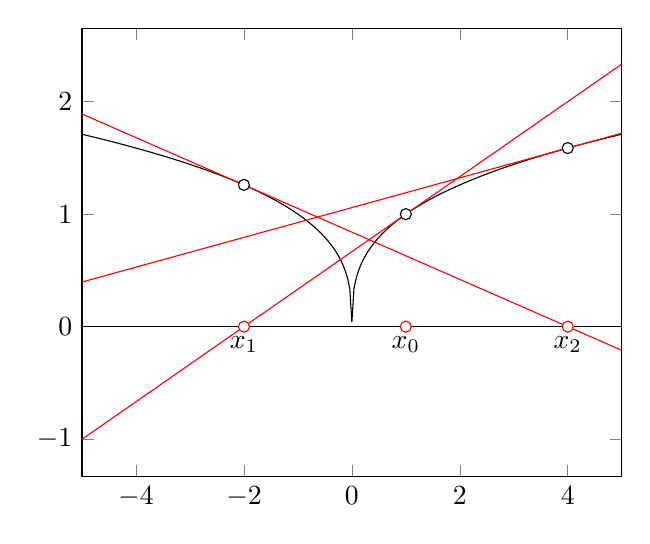
\begin{tikzpicture}
		\begin{axis}[xmin=-5, xmax=5, samples=257]
			\addplot[black] {abs(x)^(1/3)};
			\addplot[red] (x,0.33333333*x+0.666667);
			\addplot[red] (x,-0.209987*x+0.839947);
			\addplot[red] (x,0.132283*x+1.05827);
			\addplot[black] (x,0);
			\addplot[color=black,only marks,mark=*, mark options={fill=white}] 
			coordinates {
				(1, 1)
				(-2, 1.25992)
				(4, 1.5874)
			};
			\addplot[color=red,only marks,mark=*, mark options={fill=white}] 
			coordinates {
				(1, 0)
				(-2, 0)
				(4,  0)
			};
			\node [below] at (axis cs:  1, 0) {$x_0$};
			\node [below] at (axis cs:  -2, 0) {$x_1$};
			\node [below] at (axis cs:  4, 0) {$x_2$};
		\end{axis}
	\end{tikzpicture}
	\caption{Finding the root of the function $\sqrt[3]{|x|}$ using Gauss-Newton is only possible if the starting value $x_0$ is chosen as $0$, which is the root. For any other value we have that the guess gets further and further away. Indeed for any $x_n$ we have $x_{n+1} = -2x_n$.}
	\label{fig:gauss_newton_fails_cubic_root}
\end{figure}

Gauss-Newton has two problems, the starting value being too far from the root and $Dr$ not having full rank. This can be combated using the technique of dampening. Instead of moving the new guess all the way to the root of the linear approximation we only move part of the way. How far to move can be determined by a dampening factor $\lambda_n$ or a constant $\lambda$.

\subsection{Levenberg-Marquardt Algorithm}

This section is following section~18.3 of the book Introduction to Applied Linear Algebra by Stephen Boyd and Lieven Vandenberghe\cite{Boyd2018}.

As stated above, a shortcoming of Gauss-Newton is that for $x$ far from $x_n$ we must not have that $r(x) \approx r(x_n) + Dr(x_n)(x-x_n) =: \hat{r}(x, x_n)$. Levenberg-Marquardt addresses this by minimizing $||\hat{r}(x, x_n)||^2 + \lambda_n ||x-x_n||^2$. The first part is the same as above, while the second objective expresses our desire to not stray away too much from the region where we trust the linear approximation. The parameter $\lambda_n$ is a positive parameter specifying how far the trusted region extends.

Writing the above idea as a single squared norm to minimize gives us the problem

\begin{align*}
	\text{minimize }
	\left|\left|\left(\begin{matrix}
		Dr(x_n)\\ \sqrt{\lambda_n}I
	\end{matrix}\right) x - \left(\begin{matrix}
		Dr(x_n)x_n - r(x_n)\\ \sqrt{\lambda_n} x_n
	\end{matrix}\right)\right|\right|^2.
\end{align*}

We observe that as $\lambda_n$ is positive the left matrix has full rank. From this it follows that a unique solution exists.

The change of including $\lambda_n$ translates into the algorithm as replacing solving $A_n^TA_nx_{n+1} = A_n^Tb_n$ in Gauss-Newton by solving $A_n^T A_n z + \lambda_n z= A_n^T b_n + \lambda_n x_n$.

The question of how to choose $\lambda_n$ arises. If too small $x_{n+1}$ can be too far from $x_n$ to trust the approximation. If too big the convergence will be slow. If in the previous step the objective $||r(x_n)||^2$ decreased we decrease $\lambda_{n+1}$ slightly. If the last step was not successful $\lambda_n$ was too small. Therefore we increase $\lambda_{n+1}$.

Pseudo code of the resulting Levenberg-Marquardt algorithm is shown below. The stopping criteria of $||2Dr(x_n)^Tr(x_n)||$ being too small is known as the optimality condition. It is derived from the fact that $2Dr(x)^Tr(x) = \nabla||r(x)||^2 = 0$ holds for any $x$ minimizing $||r(x)||^2$. Note that this condition can be met for points other that the minimum.

\begin{algorithm}[H] \label{alg:levenberg-marquardt}
	\SetAlgoLined
	\DontPrintSemicolon
	\LinesNumbered
	\SetKwInOut{Input}{input}
	\SetKwInOut{Output}{output}
	\caption{Levenberg-Marquardt}
	
	\Input{$r: \mathbb{R}^n \rightarrow \mathbb{R}^m$ ... differentiable, $x_0 \in \mathbb{R}^n$, $\lambda_0>0$}
	\Output{$x \in \mathbb{R}^n$}
	\BlankLine
	\Begin{
		\For{$n=0$ \KwTo max\_iterations}{
			Calculate $A_n := Dr(x_n)$\;
			Calculate $b_n := A_n x_n - r(x_n)$\;
			\If{$||r(x_n)||^2$ close enough to zero or $||2A^Tr(x_n)||$ is too small}{
				break\;
			}
			Solve $(A_n^T A_n + \lambda_n) z = A_n^T b_n + \lambda_n x_n$\;
			\eIf{$||r(z)||^2 < ||r(x_n)||^2$}{
				$x_{n+1} := z$\;
				$\lambda_{n+1} := 0.8\lambda_n$\;
			}{
				$x_{n+1} := x_n$\;
				$\lambda_{n+1} := 2\lambda_n$\;
			}
		}
		$x := x_n$\;
	}
\end{algorithm}
\vspace{1cm}

Coming back to the example where Gauss-Newton failed we once again consider the function from figure~\ref{fig:gauss_newton_fails_cubic_root}. In comparison this time we are able to find a good approximation of the root using Levenberg-Marquardt. A few steps are demonstrated in figure~\ref{fig:levenberg-marquardt-example}.

\begin{figure}[h]
	\centering
	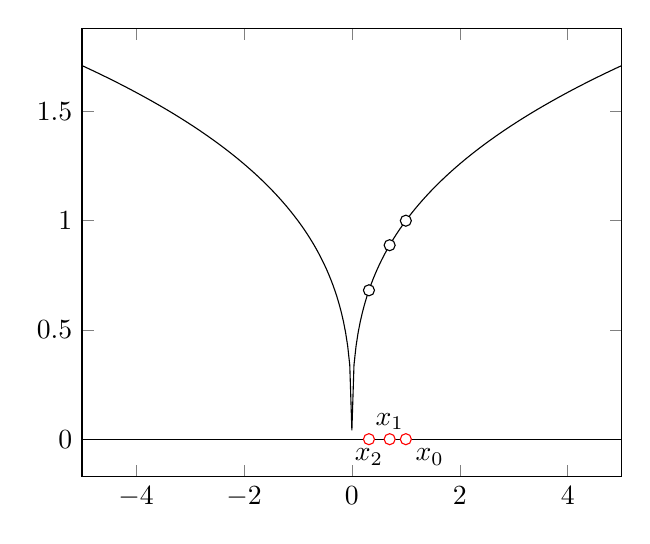
\begin{tikzpicture}
		\begin{axis}[xmin=-5, xmax=5, samples=257]
			\addplot[black] {abs(x)^(1/3)};
			\addplot[black] (x,0);
			\addplot[color=black,only marks,mark=*, mark options={fill=white}] 
			coordinates {
				(1, 1)
				(0.7, 0.887904)
				(0.316441, 0.681445)
			};
			\addplot[color=red,only marks,mark=*, mark options={fill=white}] 
			coordinates {
				(1, 0)
				(0.7, 0)
				(0.316441, 0)
			};
			\node [below right] at (axis cs:  1, 0) {$x_0$};
			\node [above] at (axis cs:  0.7, 0) {$x_1$};
			\node [below] at (axis cs:  0.316441, 0) {$x_2$};
		\end{axis}
	\end{tikzpicture}
	\caption{In comparison to Gauss-Newton, Levenberg-Marquardt is able to find the root of the function $\sqrt[3]{|x|}$. From the starting value $x_0 := 1$ and using $\lambda_0 := 1$ the guesses $x_n$ move towards the root $x=0$.}
	\label{fig:levenberg-marquardt-example}
\end{figure}

Further improvements to this algorithm can be made using good starting values perhaps from the output of other algorithms or by letting the algorithm run multiple times with different starting values and comparing the results.

\subsection{Algorithms for Bounded Least Square Problems}
\label{subsec:algorithms_bounded_lsp}

The algorithms described above do not consider bounds. For bounded problems two algorithms know as Trust Region Reflective Algorithm and Dogleg Algorithm with Rectangular Trust Regions can be used.

Trust Region Reflective gets its name from the use of trust regions as in Levenberg-Marquardt as well as reflecting along the bounds\cite{branch1999}. If an iterative $x_n$ lands outside the bounds set, it is replaced by a reflected value within the bounds. This ensures each iterative is feasible as a solution.

As the name suggests the Dogleg Algorithm with Rectangular Trust Regions uses rectangular trust regions as opposed to ellipsoids.\cite{voglis2004} As the bounds are specified as a rectangle to stay within, this results in the intersection of trust region and bounds to be rectangular. The resulting minimizing problem is solved with an adequate algorithm\cite{Nocedal1999}.

In Python the library SciPy provides the three methods Levenberg-Marquardt, Trust Region Reflective and Dogleg with Rectangular Trust Regions for solving Least Square Problems.

% https://www.applied-mathematics.net/LMvsTR/LMvsTR.pdf

% https://johnwlambert.github.io/gauss-newton/

% https://docs.scipy.org/doc/scipy/reference/generated/scipy.optimize.least_squares.html
